\chapter{Konečně projektivní roviny (KPR)}

Jistá nová struktura, která je velice symetrická a vzácná. Jedná se o množinový systém (\textbf{hypergraf} - zobecnění grafu, kde hrany mohou být k-tice. Využívá se v samoopravných kódech a přichází z geometrie.

\section{Eukleidovy axiomy}

\begin{enumerate}
	\item každé 2 body určují přímku
	\item každou úsečku lzze prodloužit na přímku
	\item ze zadaného bodu lze opsat kružnici procházejícím druhým zadaným bodem
	\item všechny pravé úhly jsou stejné
	\item bodem lze k přímce vést právě 1 rovnoběžku
\end{enumerate}

\begin{definice}[KPR]
	Konečná množina $\mathcal{X}$ a systém $\mathcal{P}$ podmnožin $\mathcal{X}$ tvoří KPR $(\mathcal{X}, \mathcal{P})$ = (body, přímky) pokud splňuje tyto tři axiomy:
	
	\begin{enumerate}
		\item $\forall x,y \in \mathcal{X}, x \neq y, \exists !P \in \mathcal{P}: \{x,y\} \subseteq P$
		\begin{itemize}
			\item každé 2 body určují právě jednu přímku
		\end{itemize}
		\item $\forall P,Q \in \mathcal{P}, P \neq Q: |P \cap Q| = 1$
		\begin{itemize}
			\item každé 2 přímky se protínají právě v 1 bodě
		\end{itemize}
		\item $\exists C \subseteq \mathcal{X}, |C| = 4, \forall P \in \mathcal{P}: |C \cap P| \leq 2$
		\begin{itemize}
			\item existují 4 body v obecné poloze
		\end{itemize}
	\end{enumerate}
\end{definice}

Jako příklad je \textbf{Fanova rovina}, která má 7 přímek a 7 bodů. Jak lze vidět na obrázku \ref{fans-plane}.

\begin{figure}[!h]\centering
	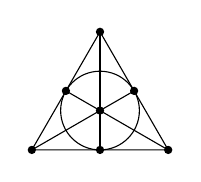
\begin{tikzpicture}
		\draw (0,0) circle (0.5);
		\draw (90:1) -- (-30:1)--(210:1)--cycle;
		\draw (90:1)--(0,0);
		\draw (210:1)--(0,0);
		\draw (-30:1)--(0,0);
		\draw (30:0.5)--(0,0);
		\draw (150:0.5)--(0,0);
		\draw (270:0.5)--(0,0);
		\fill (-0.866,-0.5) circle (1.5pt);
		\fill (0.866,-0.5) circle (1.5pt);
		\fill (0,-0.5) circle (1.5pt);
		\fill (0,1) circle (1.5pt);
		\fill (0,0) circle (1.5pt);
		\fill (0.433,0.25) circle (1.5pt);
		\fill (-0.433,0.25) circle (1.5pt);
	\end{tikzpicture}
	\caption{Fanova rovina}
	\label{fans-plane}
\end{figure}

\begin{tvrz}
	V KPR obsahuje každá přímka stejný počet bodů. $\forall P,Q \in \mathcal{P} |P|=|Q|$.
\end{tvrz}

\begin{proof}
	Empty.
\end{proof}

\begin{definice}
	Řád projektivní roviny: $(\mathcal{X}, \mathcal{P})$ je $|P|-1$ pro $P \in \mathcal{P}$.
\end{definice} 

\begin{tvrz}
	Je-li $(\mathcal{X}, \mathcal{P})$ KPR řádu $n$, pak platí:
	
	\begin{enumerate}
		\item každým bodem prochází právě $n+1$ přímek
		\item $|\mathcal{X}| = n^{2} + n + 1$
		\item$|\mathcal{P}| = n^{2} + n + 1$
	\end{enumerate}
\end{tvrz}

\begin{proof}
	Empty.
\end{proof}

\section{Dualita KPR}

"Přechod z přímek na body a z bodů na přímky."

\begin{definice}
	\textbf{Duální množinový systém} k množinovému systému $(\mathcal{X}, \mathcal{P})$ je $(\mathcal{P}, \{ \{P \in \mathcal{P} : x \in P \}: x \in \mathcal{X} \})$, zkráceně \textbf{duál}
\end{definice}

\begin{tvrz}
	Duálem KPR řádu $n$ je KPR řádu $n$.
\end{tvrz}

\begin{proof}
	Empty.
\end{proof}

\section{Existence KPR}

Kromě Fanovy roviny zatím neznáme žádné další příklady konečných projektivních rovin. Ale samozřejmě se ví o dalších které existují jmenovitě pro $(2,3,4,5,7,8,9,11)$ a $12$ už se neví. Domněnka je, že KPR řádu $n$ existuje $\Leftrightarrow$ $n$ je mocnina prvočísla. Nicméně je to pořád otevřené.

\begin{veta}
	Pokud existuje algebraické těleso o $n$ prvcích, potom existuje KPR řádu $n$.
\end{veta}

\begin{proof}
	Empty.
\end{proof}

Konstrukce funguje nad každým tělesem a například nad $\mathbb{R}$ dává \textbf{reálnou projektivní rovinu}.

\section{Latinský čtverec}

\begin{definice}
	Latinský čtverec řádu $n \in \mathbb{N}$ je tabulka $n \times n$ čísel z $\{ 1, \dots, n\}$, ve které se žádné číslo neopakuje v žádném řádku ani sloupci.
\end{definice}

\subsection{Ortogonalita}

\begin{definice}
	Latinský čtverce $L, L'$ stejného řádu jsou \textbf{ortogonální}, pokud pro každé $l, l' \in \{ 1, \dots , n\}$ existují $i,j \in \{ 1, \dots , n\}$, takové že $L_{ij} = l, L'_{ij}=l'$. Zapisuje se jako $L  \perp L'$.
\end{definice}

\begin{pozor}
	Pro ortogonální latinské čtverce $L, L'$ řádu $n$ a pár $(l,l') \in \{ 1, \dots , n\} \times \{ 1, \dots , n\}$ je pozice $(l,l')$ s $L_{ij}=l, L'_{ij}=l'$ určena jednoznačně.
\end{pozor}

\begin{proof}
	Počet párů $(l,l')$ je $n^{2}$, stejně jako počet párů $(i,j)$.
\end{proof}

\begin{pozor}
	Je-li $L = (L_{ij})_{i,j = 1}^n$ latinský čtverec a $\Pi : \{ 1, \dots , n\} \to \{ 1, \dots , n \}$ perm, tak potom $\Pi (L) := (\Pi (L_{ij})_{i,j =1}^n$ je latinský čtverec stejného řádu.
\end{pozor}

\begin{proof}
	$\Rightarrow$ BŮNO první řádek je vžzdy vzestupná řada. $\Rightarrow$ Je-li $L \perp L'$, pak $\Pi (L) \perp L'$.
\end{proof}

\begin{dusl}
	Počet \textbf{navzájem ortogonálních} nanejvýš čtverců řádu $n \in \mathbb{N}$ je $n-1$.
\end{dusl}

\begin{proof}
	Empty.
\end{proof}

\begin{veta}
	Konečná projektivní rovina řádu $n \geq 2$ existuje $\Leftrightarrow$ existuje $n-1$ navzájem ortogonálních latinských čtverců řádu $n$.
\end{veta}

\begin{proof}
	Empty.
\end{proof}
